\documentclass{beamer}

% Font selection
\usepackage{palatino}

% Beamer template
\usetheme{Antibes}
%\usetheme{Berlin}

\usepackage[scale=1.2]{ccicons}

\usepackage[utf8]{inputenc}
\usepackage[T1]{fontenc}

\usepackage{tabularx}
\usepackage{multicol}
\usepackage{graphicx}
\usepackage[final]{pdfpages}

\usepackage{listings}

\lstset{
  language=[ISO]C++,
  columns=flexible,
  identifierstyle=\itshape,
%
  belowcaptionskip=1\baselineskip,
  breaklines=true,
  xleftmargin=\parindent,
  language=C++,
  showstringspaces=false,
  basicstyle=\small,
  keywordstyle=\bfseries\color{green!40!black},
  commentstyle=\itshape\color{purple!40!black},
  identifierstyle=\color{blue},
  stringstyle=\color{brown},
  columns=flexible,
%  inputenconding=utf8,
  extendedchars=true,
%
  morekeywords=[1]{constexpr,nullptr,alignof,alignas,decltype,noexcept,override,final,concept,expects,ensures,assert},
  literate={%
    {¿}{{?`}}1
    {¡}{{!`}}1
    {á}{{\'a}}1
    {é}{{\'e}}1
    {í}{{\'i}}1
    {ó}{{\'o}}1
    {ú}{{\'u}}1
    {ñ}{{\~n}}1
}
}

\lstset{
}


\newcommand{\cppkey}[1]{%
{\color{green!40!black}\textbf{#1}}%
}

\newcommand{\cppid}[1]{%
{\color{blue}\textbf{#1}}%
}


\usepackage{tikz}
\usetikzlibrary{positioning}
\usetikzlibrary{arrows}
\usetikzlibrary{mindmap}

\usepackage{pgfplots}
\pgfplotsset{compat=1.5}


\newcommand{\textgood}[1]{%
{\color{blue}\textbf{#1}}%
}

\newcommand{\textbad}[1]{%
{\color{red}\textbf{#1}}%
}

\newcommand{\textenum}[1]{%
{\color{blue!60!black}\textbf{#1}}%
}

\newcommand{\textmark}[1]{%
{\color{orange!70!black}\textbf{#1}}%
}




% Footline in every slide
\setbeamertemplate{footline}{
  \leavevmode%
  \hbox{\begin{beamercolorbox}[wd=\paperwidth,ht=2.5ex,dp=1.125ex,leftskip=.3cm,rightskip=.3cm]{author in head/foot}%
    \usebeamerfont{author in head/foot}\ccbyncndeu 
     \quad -- \quad J. Daniel Garcia 
     -- ARCOS@UC3M (\textbf{\url{josedaniel.garcia@uc3m.es}}) 
     -- Twitter: \textbf{\url{@jdgarciauc3m}}
    \hfill
    \insertframenumber/\inserttotalframenumber
  \end{beamercolorbox}}%
  \vskip0pt%
}

% Logo in every slide
\addtobeamertemplate{headline}{}
{% 
\begin{tikzpicture}[remember picture,overlay]
\node[anchor=north east] at (current page.north east) {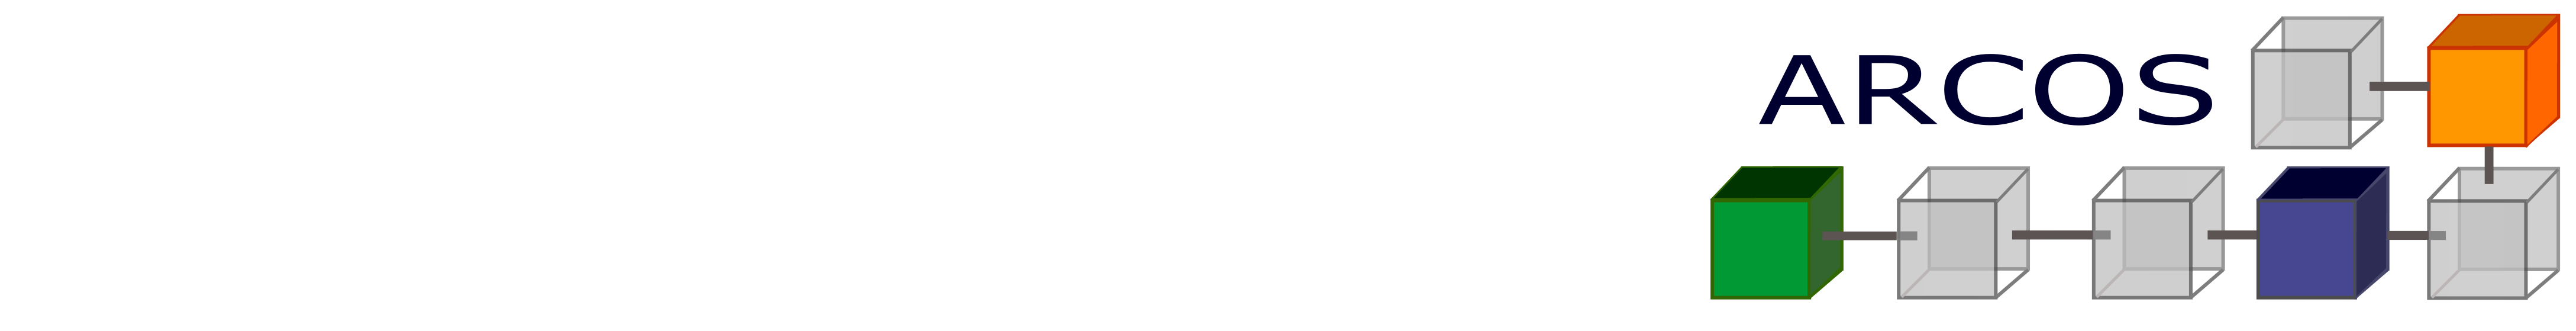
\includegraphics[height=0.7cm]{logos/arcos_t.png}};
\end{tikzpicture}
}

\tikzset{
  invisible/.style={opacity=0},
  visible on/.style={alt=#1{}{invisible}},
  alt/.code args={<#1>#2#3}{%
    \alt<#1>{\pgfkeysalso{#2}}{\pgfkeysalso{#3}} % \pgfkeysalso doesn't change the path
  },
}

%Portada
\title{Programming vulnerabilities and secure coding}
\subtitle{A language perspective}
\author{J. Daniel Garcia}
\institute{ARCOS Group\\University Carlos III of Madrid\\Spain}
\date{January, 23th 2018}

\begin{document}

\begin{frame}
\titlepage
\end{frame}

\AtBeginSection[]
{
  \begin{frame}<*>
    \setbeamertemplate{section in toc shaded}[default][50]
    \setbeamertemplate{subsection in toc shaded}[default][50]
    \tableofcontents[currentsection,hideallsubsections]
  \end{frame}
}

\AtBeginSubsection[]
{
  \begin{frame}<beamer>
    \setbeamertemplate{subsection in toc shaded}[default][50]
    \tableofcontents[currentsection,currentsubsection,hideallsubsections,,sectionstyle=show/hide,subsectionstyle=show/shaded/hide]
  \end{frame}
}

\begin{frame}{Warning}

\begin{tabularx}{.98\textwidth}{lX}
\ccLogo & This work is under 
Attribution-NonCommercial-NoDerivatives 4.0 International (CC BY-NC-ND 4.0) license.\\

& You are \textbf{free} to
\textbf{Share} — copy and redistribute the material in any medium or format.
\\

\ccAttribution & 
You must give appropriate credit, provide a link to the license, and indicate if changes were made. You may do so in any reasonable manner, but not in any way that suggests the licensor endorses you or your use.\\

\ccNonCommercialEU &
You may not use the material for commercial purposes.
\\

\ccNoDerivatives &
If you remix, transform, or build upon the material, you may not distribute the modified material.
\\

\end{tabularx}

\end{frame}

\begin{frame}{ARCOS@uc3m}
\begin{itemize}
  \item \textbf{UC3M}: A young international research oriented university.
  \vfill
  \item \textbf{ARCOS}: An applied research group.
    \begin{itemize}
      \item \textmark{Lines}: 
            High Performance Computing,
            Big data,
            Cyberphysical systems,
            \textgood{Programming Models for Applications Improvement}.
    \end{itemize} 
  \vfill
  \item \textbf{Improving applications}:
    \begin{itemize}
      \item \textmark{REPARA}: Reengineering and Enabling Performance and poweR of Applications.
            FP7-ICT (2013--2016).
      \item \textmark{RePhrase}: REfactoring Parallel Heterogeneous Resource Aware Applications.
            H2020-ICT (2015--2018).
      \item \textmark{ASPIDE}: exAScale ProgrammIng models for extreme Data procEssing.
            H2020-FET-HPC (2018--2020).
    \end{itemize} 
  \vfill
  \item \textbf{Standardization}:
    \begin{itemize}
      \item ISO/IEC JTC/SC22/WG21. ISO C++ Committee.
    \end{itemize}
\end{itemize}
\end{frame}

\section{Language Vulnerabilities Standards}

\subsection{ISO standards}

\begin{frame}[t]{ISO/IEC}
\begin{itemize}
  \item Standardization activity:
    \begin{itemize}
      \item ISO/IEC JTC1/SC22: programming languages, their environments and system software interfaces.
      \item WG23: Programming Language Vulnerabilities.
    \end{itemize}

  \vfill\pause
  \item Guidance to avoiding vulnerabilities in programming languages through language selection and use.
    \begin{itemize}
      \item ISO/IEC TR 24772:2010.
      \item ISO/IEC TR 24772:2013.
    \end{itemize}

  \vfill\pause
  \item A new series under development:
    \begin{itemize}
      \item ISO/IEC TR 24772-1
      \item \ldots
      \item ISO/IEC TR 14772-9
    \end{itemize} 
\end{itemize}
\end{frame}

\begin{frame}[t]{IS/IEC TR 14772 series}
\begin{itemize}
  \item ISO/IEC TR 24772-1 $\Rightarrow$ Language independent.
  \item ISO/IEC TR 24772-2 $\Rightarrow$ Ada.
  \item ISO/IEC TR 24772-3 $\Rightarrow$ C.
  \item ISO/IEC TR 24772-4 $\Rightarrow$ Python.
  \item ISO/IEC TR 24772-5 $\Rightarrow$ Ruby.
  \item ISO/IEC TR 24772-6 $\Rightarrow$ Spark (Ada subset).
  \item ISO/IEC TR 24772-7 $\Rightarrow$ PHP.
  \item ISO/IEC TR 24772-8 $\Rightarrow$ Fortran.
  \item ISO/IEC TR 24772-9 $\Rightarrow$ C++.
\end{itemize}
\end{frame}

\subsection{Vulnerability issues}

\begin{frame}[t]{Predictable execution}
\begin{itemize}
  \item Why doesn't software do what I expect?
    \begin{itemize}
      \item Incorrect specifications.
      \item Configuration management mistakes.
      \item \ldots
      \item Unexpected behaviour of programming language.
    \end{itemize}

  \vfill\pause
  \item What is \textmark{predictable execution}?
    \begin{itemize}
      \item Property of a program.
      \item All possible executions have results that can be predicted from examination 
            of source code.
    \end{itemize}
\end{itemize}
\end{frame}

\begin{frame}[t]{Getting predictable software}
\begin{itemize}
  \item Software may be used:
    \begin{itemize}
      \item On unanticipated platforms.
      \item On unanticipated ways.
      \item On unanticipated contexts.
      \item By unanticipated users.
    \end{itemize}

  \vfill
  \item Additionally:
    \begin{itemize}
      \item We are in a connected world.
      \item Cyberattacks!
    \end{itemize}
\end{itemize}
\end{frame}

\begin{frame}[t]{Software vulnerabilities}
\begin{itemize}
  \item \textmark{Software vulnerability}: \textbad{Unwanted} characteristic of software
        that may allow software to execute in ways that are unexpected.

    \begin{itemize}
      \item Programmers introduce vulnerabilities by using language features that are
            unpredictable.
    \end{itemize}

  \vfill\pause
  \item \textmark{Language vulnerability}: Property of a programming language that can
        contribute to application vulnerabilities.
    \begin{itemize}
      \item Security weakness.
      \item Safety hazard.
      \item Software defect.
    \end{itemize}

  \vfill\pause
  \item \textgood{Example}:
    \begin{itemize}
      \item \textbad{Language vulnerability}: String copy does not check length.
      \item \textbad{Application vulnerability}: Stack attack through buffer overrun.
    \end{itemize}
\end{itemize}
\end{frame}

\begin{frame}[t]{Sources of unpredictability}
\begin{itemize}
  \item Incomplete or evolving specifications.
  \item Undefined behaviour.
  \item Unspecified behaviour.
  \item Implementation defined behaviour.
  \item Difficult features.
  \item Inadequate language support.

  \vfill\pause
  \item Additionally:
    \begin{itemize}
      \item Porting to other platforms.
      \item Compilers might also have bugs.
      \item Use of different compiler switches.
    \end{itemize}
\end{itemize}
\end{frame}

\subsection{Rules}

\begin{frame}[t]{Rules in ISO/IEC 24772:2013}
\begin{itemize}
  \item 55 language independent rules.
    \begin{itemize}
      \item \textmark{Example}: Unchecked array copying.
    \end{itemize}

  \vfill\pause
  \item 21 application vulnerabilities.
    \begin{itemize}
      \item \textmark{Example}: Resource exhaustion.
    \end{itemize}

  \vfill\pause
  \item Informative Annexes for 6 programming languages.
    \begin{itemize}
         \item Ada.
         \item C.
         \item Python.
         \item Ruby.
         \item SPARK.
         \item PHP.
    \end{itemize}
\end{itemize}
\end{frame}

\begin{frame}[t]{Programming language vulnerabilities}
\begin{itemize}
  \item Type system: 13 rules.
  \item Conversion limits: 3 rules.
  \item Declarations and definitions: 6 rules.
  \item Operators/expressions: 4 rules.
  \item Control flow: 11 rules.
  \item Memory model: 2 rules.
  \item Generic programming: 2 rules.
  \item Libraries: 6 rules.
  \item Macros: 1 rule.
  \item Run-time: 2 rules.
  \item Language specification: 5 rules.
\end{itemize}
\end{frame}

\subsection{Summary on ISO/IEC 24772:2013}

\begin{frame}[t]{View on the TR}
\begin{itemize}

  \item Offers a catalog of vulnerabilities as well as a correspondig
        taxonomy.

  \vfill
  \item Generalization for multiple languages is difficult.

  \vfill
  \item Can be strongly biased from the perspective of some
        specific programming languages.

  \vfill
  \item Language particularization should be performed by language experts.
    \begin{itemize}
      \item One can be expert in one (or perhaps two) programming languages.
    \end{itemize}
\end{itemize}
\end{frame}




\begin{frame}
\titlepage
\end{frame}

\end{document}
